\documentclass[conference]{IEEEtran}
\usepackage[margin=1in]{geometry}
\usepackage{cite}
\usepackage{amsmath,amssymb,amsfonts}
\usepackage{algorithmic}
\usepackage{graphicx}
\usepackage{textcomp}
\usepackage{xcolor}
\usepackage{subcaption}
\usepackage{cuted}

\title{A Four Terminal Charge Pump Model Incorporating Device Leakage Effects}
\author{Mark Lipski}

\begin{document}
	\maketitle
	\section{Abstract}
	This paper constructs a steady state model of the continuous conversion ratio charge pump architecture from first principles, incorporating incomplete charge transfer and finite switch resistance. The model is then verified using a pspice model of the circuit, and the limitations of the assumptions are discussed.
	\section{Introduction}
	
	
	\section{Steady State Model}
	Most charge pump architectures can be using as a set of flying capacitors cells which switch between 4 unique voltage domains, as in Fig. \ref{Fig:SCCell}. The flying capacitor cell can then be abstracted as the four terminal device seen in Fig. \ref{Fig:SCCell_Abs}. These four terminal devices can then be used to construct various dc-dc converter configurations, such the three stage Dickson in Fig. \ref{Fig:Dickson_Block} or the series parallel converter in Fig. \ref{Fig:SeriesP_Block}.
	
	\begin{figure}
		\centering
		\begin{subfigure}{0.45\linewidth}
			\includegraphics[width=\textwidth]{Figures/SCCell.pdf}
			\caption{Switched capacitor circuit diagram.}
			\label{Fig:SCCell}	
		\end{subfigure}
	\hfill
		\begin{subfigure}{0.45\linewidth}
			\includegraphics[width=\textwidth]{Figures/SCCell_Abs.pdf}
			\caption{Switched capacitor cell abstraction.}
			\label{Fig:SCCell_Abs}	
		\end{subfigure}
	\caption{Four terminal circuit, and equivalent block level abstraction.}
	\end{figure}
	
	\begin{figure}
		\includegraphics[width=\linewidth]{Figures/Dickson.pdf}
		\caption{Three Stage Dickson configuration using four terminal devices.}
		\label{Fig:Dickson_Block}
	\end{figure}

	\begin{figure}
		\includegraphics[width=\linewidth]{Figures/SeriesParallel.pdf}
		\caption{Three Stage Series Parallel configuration using four terminal devices.}
		\label{Fig:SeriesP_Block}
	\end{figure}
	
	The internal circuit representation of the four terminal model can be seen in Fig. \ref{Fig:CircEQ}, where $R_{Fly} = \frac{1}{f_{SW}C_{Fly}}$. However, this model neglects the impact of incomplete charge transfer on the output charge delivered, which limits its usefulness.
	
	\begin{figure}
		\centering
		\includegraphics[width=0.6\linewidth]{Figures/CellRes_SSL.pdf}
		\label{Fig:CircEQ}
		\caption{Equivalent circuit model of the four terminal device operating under SSL conditions.}
	\end{figure}
	
	
	The effect of incomplete charge transfer on the output and input charge characteristics of a dc-dc converter has been studied \cite{}. However, the model studied assumed ideal clock generation. The following analysis incorporates the resistance of clock drivers into the equations for input and output current. 
	
	\subsection{Incomplete Charge Transfer}
	The associated analysis occurs at steady state  some assumptions:
	\begin{itemize}
		\item All the capacitors and resistors used in the analysis are linear and time invariant.
		\item The value of $\alpha_T + \alpha_B < 0.1$.
	\end{itemize}
	The circuit in Fig.\ref{Fig:SCCell}, can be represented as Fig. \ref{} in its first phase, with Fig. \ref{} representing its second phase. The voltage at the top and bottom plates are labeled $V_{TP}$ and $V_{BP}$ respectively, while $V_{TP1}$, would specify the top plate voltage in the first phase.
	
	The first order approximation of the voltage at $V_{TP1}$ is,
	\begin{equation}
	V_{TP1}(t) = \exp\left(\frac{-t}{\tau}\right)V_{TP1}^{i} + \left(1 - \exp\left(\frac{-t}{\tau}\right)\right)V_{T1},
	\end{equation}
	where $\tau$ is,
	\begin{equation}
	\tau = 2R_{ON}C_{Fly}\left(1+\frac{\alpha_B+\alpha_T}{2}\right),
	\end{equation}
	and $V_{TP1}^i$ is the initial value of $V_{TP1}$ at the start of the first phase. The final value of $V_{TP1}$ can be evaluated at $t = \frac{T_{SW}}{2}$, as phase 1 occupies half the period,
	\begin{equation}
	V_{TP1}^f = \exp\left\!(\tfrac{-T_{SW}}{2\tau}\right)V_{TP1}^{i} + \left(1 - \! \exp\!\left(\tfrac{-T_{SW}}{2\tau}\right)\right)V_{T1}.
	\end{equation}	
	Finally, a substitution can be made, relating to the exponential decay at the end of the time step,
	\begin{equation}
	A = \exp\left(-\tfrac{T_{SW}}{2\tau}\right) = \exp\left(\tfrac{T_{SW}}{2R_{ON}C_{Fly}\left(2+\alpha_B+\alpha_T\right)}\right),
	\end{equation}
	which can be used to create a simplified expression for $V_{TP1}^f$,
	\begin{equation}
	V_{TP1}^f = AV_{TP1}^i + (1-A)V_{T1}.
	\end{equation}
	A similar procedure can then be repeated for the other nodal voltages,
	\begin{equation}
	V_{BP1}^f = AV_{TP1}^i + (1-A)V_{B1},
	\end{equation}
	\begin{equation}
	V_{TP2}^f = AV_{TP2}^i + (1-A)V_{T2},
	\end{equation}
	\begin{equation}
	V_{BP2}^f = AV_{BP2}^i + (1-A)V_{B2}.
	\end{equation}
	
	The initial conditions of $C_{Fly}$ at the start of each phase can be acquired using the voltage stored on the capacitor. The voltage stored on the capacitor at the end of any phase is $V_{TPx} - V_{BPx}$, where $x$ is the phase. Using the voltage on the capacitor, the initial conditions can be constructed, 
	\begin{equation}
	V_{TP1}^i = \tfrac{V_{TP2}^f - V_{BP2}^f + V_{T1} + V_{B1}}{2},
	\end{equation}
	\begin{equation}
	V_{BP1}^i = \tfrac{V_{BP2}^f - V_{TP2}^f + V_{B1} + V_{T1}}{2},
	\end{equation}
	\begin{equation}
	V_{TP2}^i = \tfrac{V_{TP1}^f - V_{BP1}^f + V_{T2} + V_{B2}}{2},
	\end{equation}
	\begin{equation}
	V_{BP2}^i = \tfrac{V_{BP1}^f - V_{TP1}^f + V_{T2} + V_{B2}}{2}.
	\end{equation}
	Using the equations for the initial conditions and the final voltages, the final voltages can be solved,
	\begin{equation}
	V_{TP1}^f = V_{T1} + \Delta V, 
	\end{equation}
	\begin{equation}
	V_{BP1}^f = V_{B1} - \Delta V,
	\end{equation}
	\begin{equation}
	V_{TP2}^f = V_{T2} - \Delta V,
	\end{equation}
	and
	\begin{equation}
	V_{BP2}^f = V_{B2} + \Delta V
	\end{equation}
	where 
	\begin{equation}
	\Delta V = \frac{A(V_{B1} - V_{T1} - V_{B2} + V_{T2})}{2(A+1)}.
	\end{equation}
	This can then be used to generate the circuit model seen in Fig. \ref{Fig:Circ_Res}, which will incorporate the effects of incomplete charge transfer.
	
	\begin{figure}
		\centering
		\includegraphics[width=0.7\linewidth]{Figures/CellRes.pdf}
		\caption{Four terminal device model incorporating switch resistance.}
		\label{Fig:Circ_Res}
	\end{figure}

	This can then be verified using an ideal model of the circuit, using both a single SC cell, and in more complex configurations, such as the Dickson and series parallel. The resulting comparison can be seen in Fig. \ref{}, where the resistance and voltage are held constant, and the frequency is varied.
	
	A second set of tests was run to verify that the impact of $\alpha_B$ and $\alpha_T$ was as predicted, which can be seen in Fig. \ref{}.
	
	\subsection{Leakage Effects}
	The leakage effects associated with the transistors are modelled using theory from the \cite{} transistor models. The testing is performed in pspice, using the PTM to simulate the transistors used. 
	
	
\end{document}